\documentclass[5p,times,authoryear]{elsarticle}

\usepackage{ecrc}
\usepackage{amsmath}
\usepackage{amsfonts}
\usepackage{amssymb}
\usepackage{subcaption}
\usepackage[title]{appendix}
\usepackage{titlesec}
\usepackage{xcolor}
\usepackage{mathtools}
\usepackage{amsthm}
\newtheorem{proposition}{Proposition}
\newtheorem{theorem}{Theorem}
\AtBeginDocument{\renewcommand{\harvardand}{\&}}
\setcitestyle{authoryear,open={(},close={)}}
\usepackage[figuresright]{rotating}
\usepackage{tikz}
\usetikzlibrary{arrows.meta,positioning,shapes.geometric,shapes.misc,shapes.symbols,calc,backgrounds,fit}
\usepackage[colorlinks=true,citecolor=blue,linkcolor=blue,urlcolor=blue]{hyperref}
\usepackage{cleveref}

\volume{00}
\firstpage{1}
\journalname{Control Engineering Practice}
\runauth{}
\jid{procs}

\begin{document}

\begin{frontmatter}
\dochead{}

\title{Robust Cradle Recovery of an Underactuated USV via Reach Avoid Reachability}

\author{Kiyong Park}
\ead{qkrrldyd777@kaist.ac.kr}
\author{Jinwhan Kim\corref{cor1}}
\ead{jinwhan@kaist.ac.kr}
\cortext[cor1]{Corresponding author.}
\address{Department of Mechanical Engineering, Korea Advanced Institute of Science and Technology (KAIST), Daejeon 34141, Republic of Korea}

\begin{abstract}
This paper presents a robust cradle recovery framework based on reach avoid reachability for docking an underactuated unmanned surface vehicle (USV) into a cradle on the side of a moving mothership. Autonomous recovery is challenging because the underactuated USV must approach and enter a narrow cradle that advances with the mothership, without colliding with the hull or the cradle structure, while wind, wave, and current disturbances act on it. Safe and effective recovery therefore requires a controller that guarantees both collision avoidance and arrival at the recovery point, and Hamilton Jacobi reachability, in particular its reach avoid formulation, provides this guarantee by characterizing the set of states from which the USV can be driven into the cradle while avoiding collision under the worst case disturbance, together with the optimal control input that achieves it. Conventional dynamic programming solvers of this set are intractable in the high dimensional state space of a full USV model, whereas reinforcement learning makes the computation feasible. Building on this, the recovery set is learned through a robust reinforcement learning scheme, and a two phase recovery system is proposed, in which a disturbance observer based model predictive controller drives the USV during the approach from a far distance and the learned policy takes over to complete the recovery once the state enters the set. Numerical simulations and processor in the loop experiments demonstrate robust and collision free recovery under environmental disturbances.
\end{abstract}

\begin{keyword}
Unmanned surface vehicle \sep autonomous recovery \sep reach avoid \sep reinforcement learning \sep Hamilton Jacobi reachability \sep safe learning
\end{keyword}

\end{frontmatter}

\section{Introduction}\label{sec_intro}

Collaborative maritime systems pair a large mothership with small unmanned surface vehicles (USVs) that perform missions such as surveillance, search and rescue, and environmental monitoring. Such systems follow a marsupial architecture, in which the mothership deploys and retrieves the USVs through a launch and recovery system (LARS). Since the USVs are unmanned, the recovery must also be performed autonomously for the concept to be practical. In field operations the mothership is kept underway rather than stopped during recovery. Maintaining forward speed keeps the ship on a steady course and gives the approaching craft the relative flow it needs for directional control. In particular, recovery is more demanding than launch, due to its sensitivity to the sea state and the operator skill it requires \citep{sheinberg2003stern, sheinberg2010operational, chun2012experimental}. Recovery is commonly performed either through a stern ramp or into a side mounted cradle. This work adopts the side cradle, because the USV can then approach in the sheltered lee along the full length of the hull, where the incident waves are strongly attenuated, and remain clear of the mothership's propeller wash and stern wake, which make stern recovery difficult. The paper therefore addresses the automated recovery of a USV into such a cradle on a mothership that is underway.

Autonomous recovery into such a cradle is a demanding control problem. The USV is underactuated, driven by a single stern thruster and a rudder, so sway is unactuated and the thrust and rudder rates are limited. With this restricted authority it must align in position and heading and enter a narrow cradle pocket that advances continuously with the mothership, avoiding collision with the hull and the cradle structure, all under persistent wind, wave, and current disturbances.

Safe and effective recovery therefore requires a controller that guarantees two properties at once, collision avoidance during the approach and arrival at the cradle. A range of robust and safety oriented control methods are relevant to this goal, yet each leaves a gap for the present task. Robust and tube model predictive control guarantees recursive feasibility and convergence to a robust invariant set around the reference when terminal ingredients and a robust invariant tube are available \citep{langson2004tube, mayne2005robust}. For a nonlinear underactuated vessel with actuator amplitude and rate limits, however, these ingredients must be constructed offline over the maneuvering envelope and are conservative, so the guaranteed set of initial states can be much smaller than the true set of states from which recovery is possible. Disturbance observer based control, including L1 adaptive control \citep{hovakimyan2010l1} and disturbance observer based model predictive control \citep{park2026recovery, tomera2021dob}, estimates and compensates the environmental load and improves tracking, but it addresses disturbance rejection rather than guaranteeing that the USV can reach the cradle without collision. Control barrier functions enforce safety as forward invariance and can be made robust to bounded disturbances \citep{xu2015robustness}, and embedding such barrier constraints in model predictive control imposes safety across the prediction horizon \citep{zeng2021safety, zeng2021enhancing}. Even so, recursive feasibility of the resulting program is not guaranteed under underactuation and actuator saturation, where the admissible safe input set can become empty before the cradle is reached.

Hamilton Jacobi reachability, in particular its reach avoid formulation, directly provides the missing guarantee \citep{margellos2011hamilton, bansal2017hamilton}. The reach avoid set characterizes exactly those states from which the USV can be driven into the cradle while avoiding collision under the worst case admissible disturbance, and the associated value function yields the optimal control input that achieves this outcome. Membership in the reach avoid set is therefore a certificate that an admissible recovering input exists at every instant along the remaining maneuver, which is precisely the property that the barrier based methods cannot ensure.

Computing this set is the remaining obstacle. Classical grid based dynamic programming solvers of the reach avoid value discretize the state space and suffer from the curse of dimensionality \citep{mitchell2005time}, so they are intractable for the full state of the USV. Reinforcement learning removes this bottleneck by approximating the reach avoid value function and its policy with neural networks at this scale \citep{bansal2021deepreach, fisac2019bridging, hsu2021safety}, and formulating the learning problem as a bounded disturbance game between control and disturbance is what makes the resulting set robust rather than merely nominal.

This paper builds on these observations and proposes a certified two phase recovery system for cradle recovery of an underactuated USV. A reach avoid set and its policy must be computed over the whole state domain in advance, which is costly over the large region that a full recovery spans, from the distant approach to the narrow cradle entry, so applying reachability to the entire recovery would be inefficient. The recovery is therefore split. A disturbance observer based model predictive controller drives the USV over the long approach \citep{park2026recovery}, where the region is large but the maneuver is mild, and the reach avoid set with its robust policy is reserved for the terminal docking, where the region is small but safety is critical. To this end the reach avoid problem, comprising the target set, the avoid set, and the augmented state, is formulated specifically for the USV dynamics and the moving cradle, and a robust reinforcement learning scheme learns the resulting set and policy under bounded disturbances. Once the measured state enters the learned set, the policy takes over and completes the docking, and set membership certifies both sides of the switch, triggering the handoff into docking.

The main contributions of this paper are summarized as follows.
\begin{enumerate}\itemsep=0pt
\item A robust reach avoid formulation of USV cradle recovery that encodes collision avoidance with the mothership and the cradle together with the amplitude and rate limits of the underactuated USV.
\item A robust reach avoid set and policy obtained by reinforcement learning under a bounded disturbance adversary, certifying a recovering input over the full USV state where grid based reachability is intractable.
\item A reachability based two phase recovery framework that assigns a controller suited to each phase and uses reach avoid set membership as a certified handoff between them.
\end{enumerate}
The rest of the paper is structured as follows. Section 2 reviews related work. Section 3 describes the USV model. Section 4 formulates the recovery problem. Section 5 presents the control system design. Section 6 reports the results. Section 7 concludes the paper.

\section{Related Work}\label{sec_related}

\textit{Autonomous docking, berthing, and marine recovery.} Autonomous launch and recovery of marine vehicles has been studied mostly for underwater vehicles returning to a surface or subsea platform, using waypoint and acoustic homing guidance validated at sea \citep{sarda2019launch}, layered model free adaptive control of the recovery vessel \citep{liao2023disturbance}, and observer based backstepping sliding mode docking of an underactuated vehicle \citep{xie2022threedimensional, yazdani2020underwaterdocking, zhang2023uuvrecovery}. Recovery of a surface vehicle into a moving mothership has been treated with kinematic path planning \citep{xu2023multistage} and with disturbance observer based model predictive control under reach avoid barriers \citep{park2026recovery}, and reachability analysis has been applied to the approach toward a static berth \citep{park2020reachability}. Recovery also arises on other platforms, including aerial landing on a moving ship deck by visual servoing \citep{cho2022shipdeck}, fixed wing net recovery \citep{singh2024sdre}, and spacecraft rendezvous and docking \citep{luo2014rendezvous}, where recovery onto a moving host is the difficult case. For an underactuated surface vehicle entering a moving cradle under disturbance, existing methods do not certify that an admissible input keeps it clear of the mothership and the cradle while still reaching the pocket.

\textit{Robust and safe control.} Robust and tube based model predictive control keeps the state within a tube around a nominal trajectory and provides recursive feasibility and convergence to a robust invariant set when terminal ingredients are available \citep{langson2004tube, mayne2005robust}, but this invariant set is hard to construct and conservative for a nonlinear underactuated vessel whose actuation is limited in both amplitude and rate. Disturbance observer based model predictive control incorporates the estimated disturbance into the prediction model \citep{tomera2021dob}, while L1 augmented model predictive control runs an L1 adaptive law in parallel with the predictive controller \citep{hovakimyan2010l1}, yet for an underactuated nonlinear vessel it is hard to guarantee recursive feasibility while also enforcing collision avoidance. Control barrier functions enforce forward invariance of a safe set and can be made robust to bounded perturbations \citep{xu2015robustness}, with related robust control barrier value functions \citep{choi2021robust}, and they have been embedded as constraints in model predictive control \citep{zeng2021safety, zeng2021enhancing, wang2025safety}. These methods are mostly avoidance oriented and enforce safety one step at a time, so they do not guarantee reaching a moving target and can lose recursive feasibility under underactuation and actuator saturation.

\textit{Hamilton Jacobi reachability and reinforcement learning.} Hamilton Jacobi reachability computes a backward reachable set, the states from which a target is reached or a failure set avoided under the worst case disturbance, as the sublevel set of a value function that solves a partial differential equation \citep{lygeros2004reachability, mitchell2005time}, and the reach avoid extension combines the two \citep{margellos2011hamilton, fisac2015reach}. Grid based solvers are convergent but scale exponentially with dimension \citep{mitchell2008toolbox}. DeepReach scales to higher dimension with a self supervised neural solver of this equation that returns a value and its induced controller, and whose value can be verified or corrected for formal assurances \citep{bansal2021deepreach, lin2023generating, lin2024verification, singh2025exact}. Learned reach avoid values have moved beyond analysis into closed loop control, deployed as safety and liveness filters wrapped around nominal controllers and validated on hardware \citep{borquez2024safety, nguyen2024gameplay, lin2026onefilter}, and a learned value can itself be formally verified for accuracy \citep{yang2025scalable}. As another approach, reachability has been recast as reinforcement learning, learning the value and the policy from rollouts through a discounted safety backup that is a contraction \citep{fisac2019bridging}, extended to reach avoid objectives \citep{hsu2021safety}, to feasible set and performance constrained formulations \citep{yu2022reachability, ganai2023respo}, and to robust two player settings where a worst case disturbance acts as a second player \citep{hsu2023isaacs, li2023robust}. We build on this line, learning the robust reach avoid value and a deployable policy from rollouts within a single framework.

\section{Dynamic Modeling of Surface Vehicles}\label{sec_model}

The USV is described by a three degree of freedom maneuvering model in surge, sway, and yaw, following standard marine craft hydrodynamics \citep{fossen2011handbook}. The world frame and the body frame are shown in Fig.~\ref{fig_coordinate}. The USV carries a single stern thruster with a rudder, so the sway direction is unactuated.

\begin{figure}[t]
\centering
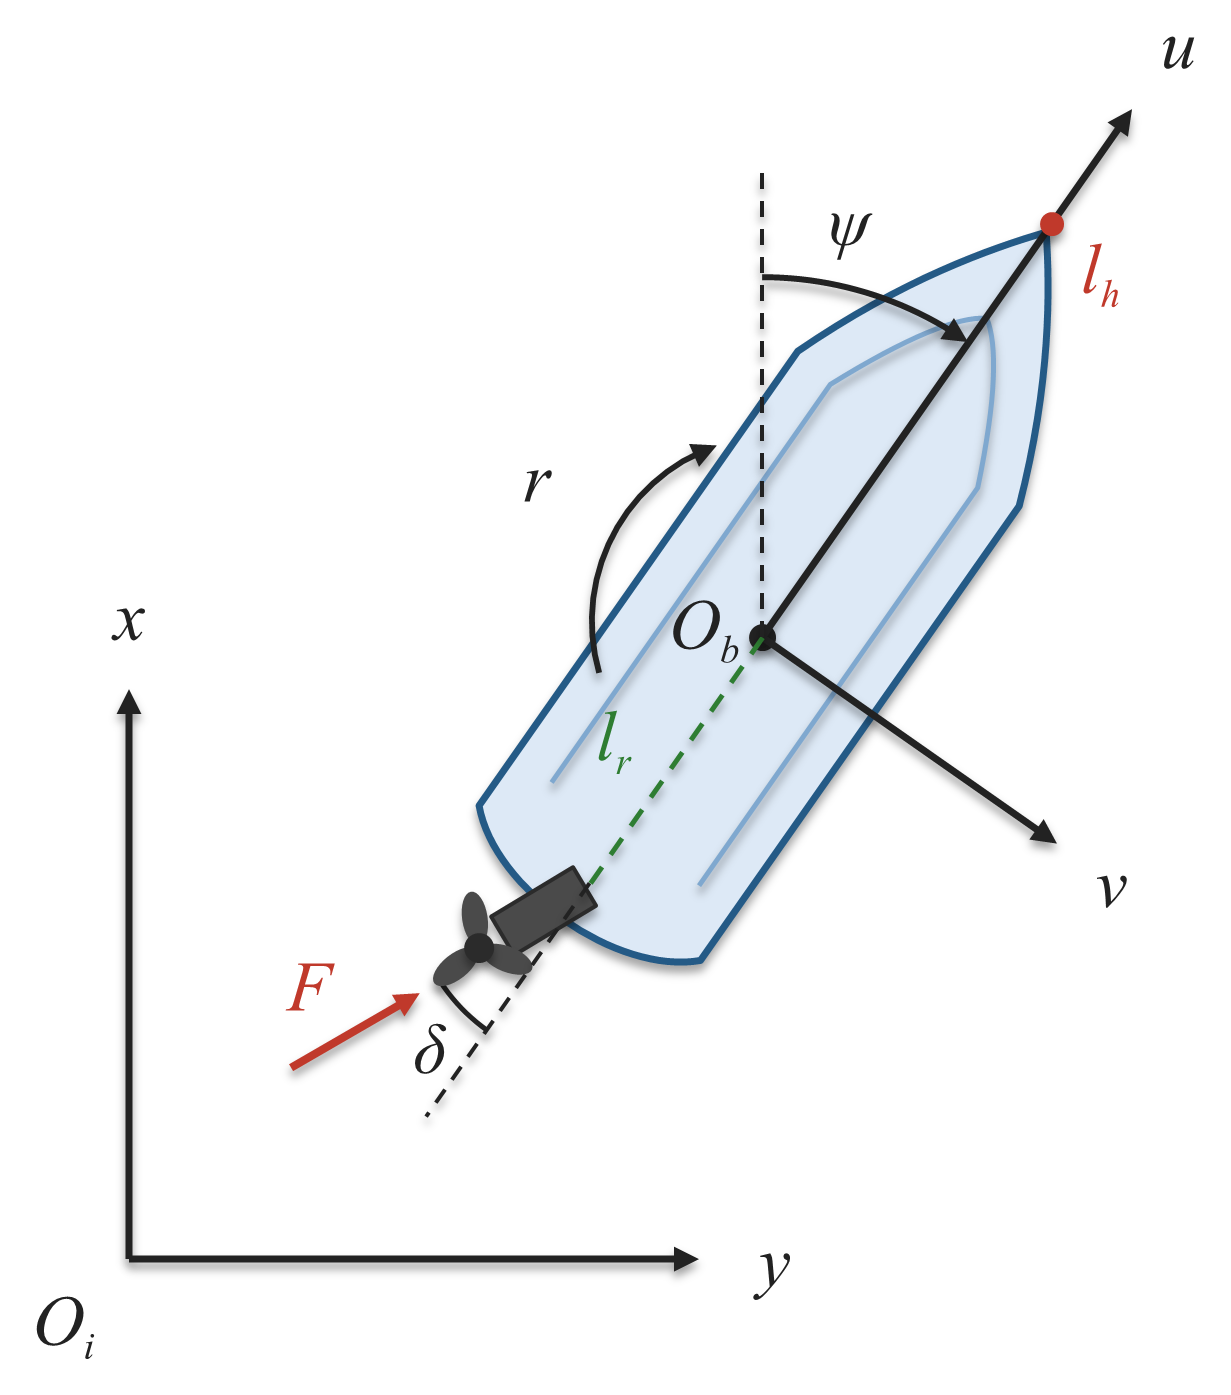
\includegraphics[width=0.6\linewidth]{fig/coordinate_frame}
\caption{Coordinate frames and actuator geometry of the USV.}
\label{fig_coordinate}
\end{figure}

The kinematics relate the body frame velocity $\nu = [u, v, r]^\top$ to the world frame pose $\eta = [x, y, \psi]^\top$ through the yaw rotation.
\begin{equation}\label{eq_kin}
\dot\eta = R(\psi)\,\nu,\qquad
R(\psi) = \begin{bmatrix} \cos\psi & -\sin\psi & 0 \\ \sin\psi & \cos\psi & 0 \\ 0 & 0 & 1 \end{bmatrix}.
\end{equation}
The kinetics in the body frame follow the standard maneuvering model.
\begin{equation}\label{eq_kinetics}
M\dot\nu + C(\nu)\,\nu + D(\nu)\,\nu = \tau_c + \tau_w,
\end{equation}
where $M$ is the inertia matrix, $C(\nu)$ the Coriolis matrix, $D(\nu)$ the damping matrix, $\tau_c = [\tau_u, \tau_v, \tau_r]^\top$ the control force and moment, and $\tau_w = [w_u, w_v, w_r]^\top$ the environmental disturbance force. The matrices are given as follows.
\begin{subequations}\label{eq_matrices}
\begin{align}
M &= \begin{bmatrix} m_{11} & 0 & 0 \\ 0 & m_{22} & 0 \\ 0 & 0 & m_{33} \end{bmatrix}, \\[2pt]
C(\nu) &= \begin{bmatrix} 0 & 0 & -m_{22} v \\ 0 & 0 & m_{11} u \\ m_{22} v & -m_{11} u & 0 \end{bmatrix}, \\[2pt]
D(\nu) &= -\begin{bmatrix} X_u & 0 & 0 \\ 0 & Y_v & Y_r \\ 0 & N_v & N_r \end{bmatrix} \nonumber \\
&\quad -\begin{bmatrix} X_{u|u|}|u| & 0 & 0 \\ 0 & Y_{v|v|}|v| & Y_{r|r|}|r| \\ 0 & N_{v|v|}|v| & N_{r|r|}|r| \end{bmatrix},
\end{align}
\end{subequations}
where $m_{11}=m-X_{\dot u}$, $m_{22}=m-Y_{\dot v}$, and $m_{33}=I_z-N_{\dot r}$ include the added mass and added moment of inertia, the first bracket of $D(\nu)$ collects the linear drag coefficients, and the second collects the quadratic drag coefficients.

The USV is actuated by a single stern thruster of thrust $F$ deflected by the rudder angle $\delta$, so the control force and moment are the projection of the thrust onto the body axes.
\begin{equation}\label{eq_actuator}
\tau_c = \begin{bmatrix} \tau_u \\ \tau_v \\ \tau_r \end{bmatrix} = \begin{bmatrix} F\cos\delta \\ F\sin\delta \\ -\,l_r\,F\sin\delta \end{bmatrix},
\end{equation}
where $l_r$ is the distance from the center of gravity to the thruster. The identified parameter values are listed in Table~\ref{tab_params} in Section~\ref{sec_results}.

The rudder and thrust are bounded in amplitude, and their rates are bounded as well, so the admissible input sets are the following.
\begin{equation}\label{eq_amp}
\mathcal{U} = \big\{\, (\delta, F) \,\big|\, \delta_{\min}\le \delta\le \delta_{\max},\ F_{\min}\le F\le F_{\max} \,\big\},
\end{equation}
\begin{equation}\label{eq_rate}
\dot{\mathcal{U}} = \big\{\, (\dot\delta, \dot F) \,\big|\, \dot\delta_{\min}\le \dot\delta\le \dot\delta_{\max},\ \dot F_{\min}\le \dot F\le \dot F_{\max} \,\big\}.
\end{equation}


\begin{figure*}[t]
\centering
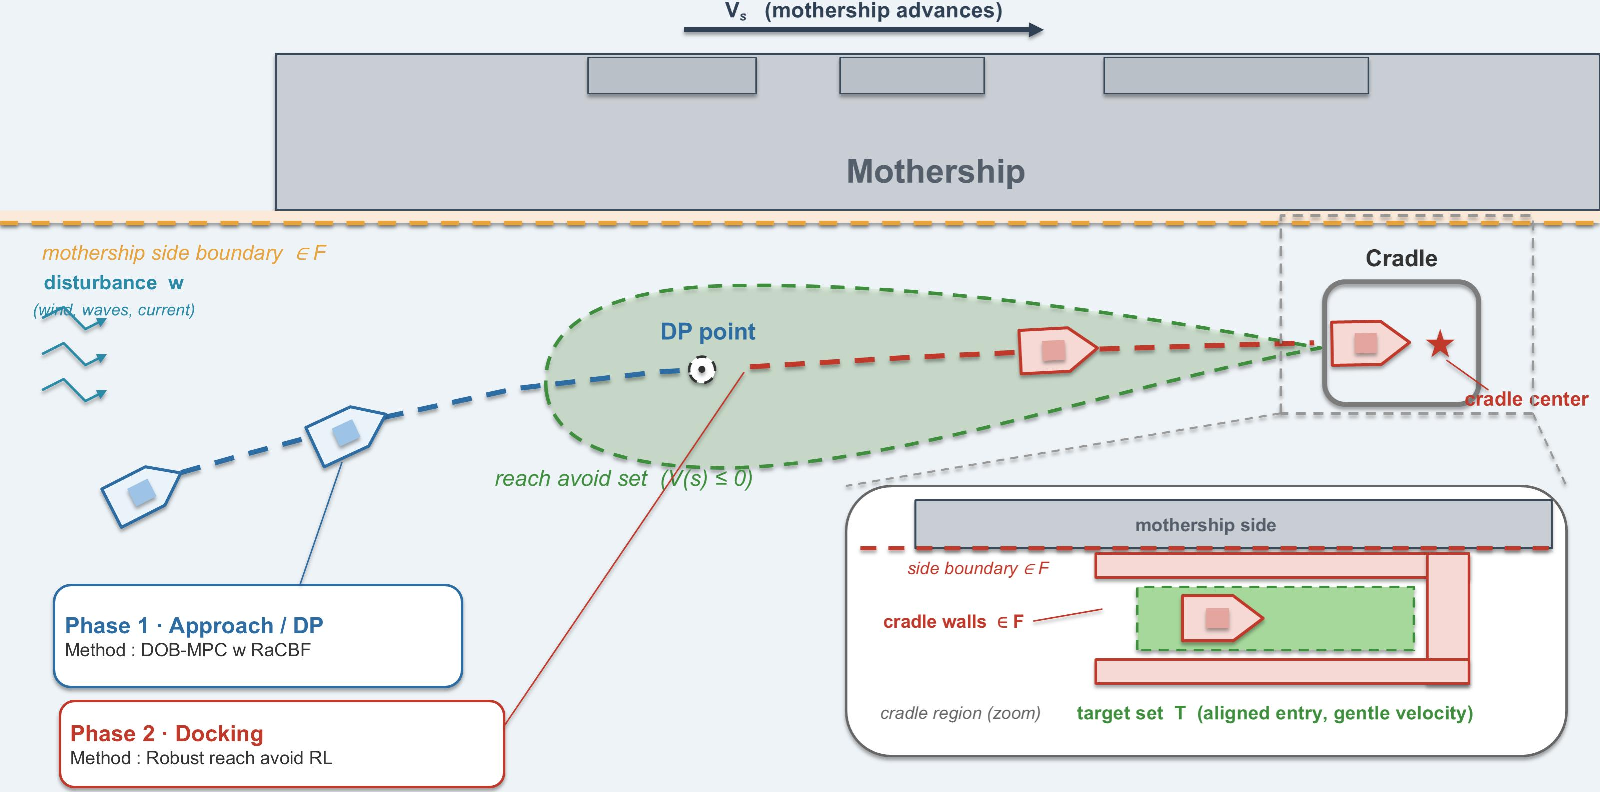
\includegraphics[width=\linewidth]{fig/recovery_scenario}
\caption{Top view of the recovery scenario. The mothership advances at the stream speed $V_s$ while the USV executes the two phase recovery, first holding the dynamic positioning point and then docking from within the reach avoid set of the learned policy, and the zoom inset marks the target set inside the cradle and the surrounding collision set.}
\label{fig_scenario}
\end{figure*}


\section{Problem Formulation}\label{sec_problem}

The recovery task is illustrated in Fig.~\ref{fig_scenario}. An underactuated USV approaches from alongside the mothership and must enter the side cradle matched in position and heading, without striking the mothership hull or the cradle structure. Wind, wave, and current disturbance act on the vehicle throughout, and the cradle advances with the mothership at the stream speed $V_s$.

The problem is posed in a cradle fixed frame that advances with the mothership at $V_s$. Because the mothership is far larger and heavier than the USV, it maintains a steady heading and its motion is negligible over the recovery, and the crane stabilises the cradle against ship motion, so in this frame the cradle is nearly stationary. The state $s = [x_r, y_r, \psi_r, u, v, r, \delta, F]^\top \in \mathbb{R}^8$ collects the relative pose, the velocity, and the actuator states, the control is the pair of actuator rates $a = [\dot\delta, \dot F]^\top$, and the disturbance $w \in \mathcal{W}$ is bounded as in Section~\ref{sec_model}. Two sets describe the outcome through scalar margin functions $\ell$ and $g$,
\begin{equation}\label{eq_margins}
\ell(s)\le 0 \iff s\in\mathcal{T},\qquad g(s)>0 \iff s\in\mathcal{F},
\end{equation}
evaluated at two points on the USV, the center of gravity and the head point, a reference point at the bow a fixed distance forward of the center of gravity. The target set $\mathcal{T}$ requires the head point to enter the cradle pocket with the heading close to the cradle direction and a gentle relative velocity. The head point crosses the cradle mouth before the center of gravity does, and once it is inside the cradle, plain forward thrust alone draws the rest of the hull in after it. Reaching $\mathcal{T}$ with the head point, together with a heading aligned to the cradle, therefore already marks a docking that will complete, which is why the head point rather than the whole body is what must reach $\mathcal{T}$. The failure set $\mathcal{F}$ collects every state in which either the center of gravity or the head point strikes the mothership hull or the cradle structure, so both points must stay clear. Both sets are marked in the zoom inset of Fig.~\ref{fig_scenario}, and the concrete geometry and numeric thresholds appear in Section~\ref{sec_results}.

The objective is to drive the USV so the head point reaches $\mathcal{T}$ while neither the center of gravity nor the head point ever enters $\mathcal{F}$, for every admissible disturbance, which defines a robust reach avoid problem.

\section{Control System Design}\label{sec_control}

\subsection{Recovery Framework}\label{sec_framework}
\begin{figure}[t]
\centering
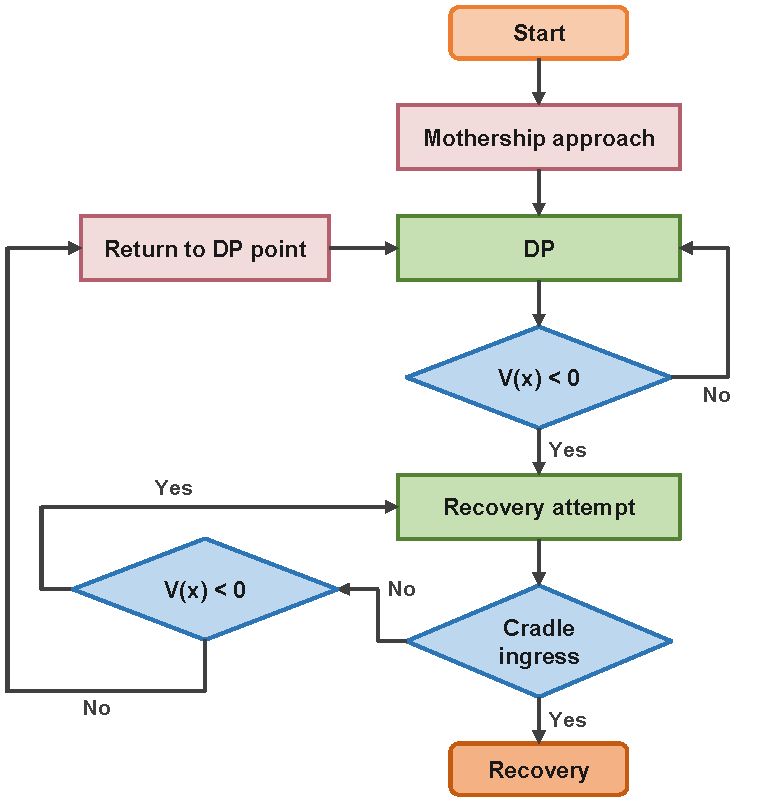
\includegraphics[width=0.9\linewidth]{fig/recovery_flowchart}
\caption{Recovery state machine. Phase 1 holds the DP point and hands control to the Phase 2 reach avoid policy once the state enters the learned set, and control falls back to Phase 1 if the state leaves the set before the cradle is entered.}
\label{fig_flowchart}
\end{figure}


The recovery runs in two phases, shown in Fig.~\ref{fig_scenario}. The reach avoid set must be computed over the whole region of states it is to cover, so relying on it for the far approach would be inefficient over such a large region, and far from the cradle there is relatively little to avoid. For these reasons Phase 1, the long approach and the dynamic positioning alongside the mothership, uses a disturbance observer based model predictive controller (DOB-MPC) with a robust adaptive control barrier function (RaCBF) \citep{park2026recovery}, in which the disturbance observer estimates the environmental disturbance, the DOB-MPC rejects it while respecting the actuator amplitude and rate limits over a horizon, and the RaCBF keeps the USV from colliding with the mothership. Near the cradle the situation is harsh, the cradle is narrow, the disturbance acts, and the USV is underactuated with actuation limits, so a guarantee of safe recovery is needed. Phase 2, the terminal docking, is therefore carried out by the robust reach avoid policy of Section~\ref{sec_rl}, whose certified set covers this terminal region.

The two phases are connected by a supervisor, whose state machine is shown in Fig.~\ref{fig_flowchart}. The Phase 2 policy of Section~\ref{sec_rl} carries the value function $V$ of the Hamilton Jacobi reach avoid problem, and the reach avoid set is where $V(s)<0$. From such a state the USV can reach the target and avoid the failure set under the worst case disturbance, and a state with $V(s)\ge 0$ lies outside the set. Phase 1 first brings the USV to the vicinity of the dynamic positioning point, and the supervisor then begins to test the sign of $V(s)$. When $V(s)<0$ it hands control to the Phase 2 policy, and control falls back to Phase 1 when $V(s)\ge 0$ before the cradle is entered, so a single scalar test governs both the transition and the abort. A disturbance larger than predicted can arrive suddenly, or a communication or mechanical fault can occur, and either can drive the state out of the reach avoid set during docking, so the sign test returns control to Phase 1 and the approach is retried.

\subsection{Robust Reach Avoid Reinforcement Learning}\label{sec_rl}
The reach avoid recovery problem posed earlier is naturally solved by Hamilton Jacobi reachability analysis \citep{mitchell2005time, bansal2017hamilton, lygeros2004reachability}. The USV is underactuated with a single stern thruster and a rudder, it faces a bounded environmental disturbance, and it must reach a cradle that moves with the mothership while avoiding collision. This casts recovery as a two player differential game in which the control minimises a value and the bounded disturbance maximises it. The value assigns to every state a number, and the states where this number is at most zero form the set of interest.

\begin{figure*}[t]
  \centering
  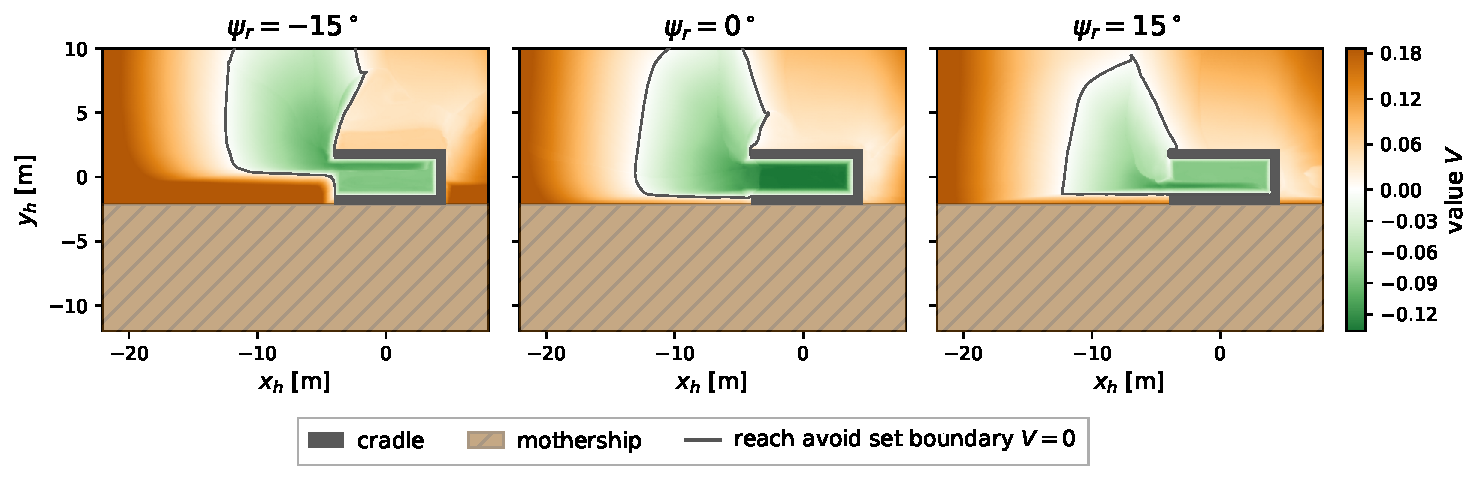
\includegraphics[width=\linewidth]{fig/reach_avoid_set}
  \caption{Learned robust reach avoid set at three headings and the docking speed. The shaded region where the value $V$ is negative is the set of states from which the trained policy recovers the USV, bounded by its zero level and clear of the mothership.}
  \label{fig_set}
\end{figure*}

The reach avoid problem asks the system to reach the target set $\mathcal{T}$ while never entering the failure set $\mathcal{F}$, under the worst case disturbance \citep{margellos2011hamilton, fisac2015reach, hsu2021safety}. Let $\xi^{a}_s(\cdot)$ denote the state trajectory from $s$ under the control $a$, and let $\tau$ and $\kappa$ be times. With the target margin $\ell$ and the failure margin $g$ of \eqref{eq_margins}, the reach avoid outcome of a trajectory is the payoff, and the value is its optimum over the control.
\begin{equation}\label{eq_payoff}
\begin{aligned}
V^{a}(s) &= \min_{\tau\ge 0}\, \max\Big\{ \ell\big(\xi^{a}_s(\tau)\big),\ \max_{\kappa\in[0,\tau]} g\big(\xi^{a}_s(\kappa)\big) \Big\}, \\
V(s) &= \inf_{a} V^{a}(s).
\end{aligned}
\end{equation}
The value is negative exactly on the reach avoid set $\mathrm{RA}(\mathcal{T},\mathcal{F})$, the states from which the control can steer the trajectory into $\mathcal{T}$ while keeping it clear of $\mathcal{F}$, that is $V(s)\le 0 \iff s\in\mathrm{RA}(\mathcal{T},\mathcal{F})$. Dynamic programming turns \eqref{eq_payoff} into the reach avoid Bellman equation \citep{hsu2021safety}, with $s'$ the next state.
\begin{equation}\label{eq_rabe}
V(s) = \max\Big\{ g(s),\ \min\big\{ \ell(s),\ \inf_{a} V(s') \big\} \Big\}.
\end{equation}
This Bellman equation was solved classically by grid based dynamic programming, but such solvers scale exponentially with the state dimension and cannot be applied to the eight dimensional state of Section~\ref{sec_model}, which motivates the learning based method developed next. A discount $\gamma\in[0,1)$ makes the backup a contraction \citep{fisac2019bridging, hsu2021safety}. This is the discounted reach avoid Bellman equation.
\begin{equation}\label{eq_drabe}
\begin{aligned}
V_\gamma(s) = {}& (1-\gamma)\max\{\ell(s), g(s)\} \\
&+ \gamma\,\max\Big\{ g(s),\ \min\big\{ \ell(s),\ \inf_{a} V_\gamma(s') \big\} \Big\}.
\end{aligned}
\end{equation}
Related reachability constrained formulations appear in \citet{yu2022reachability}.

The proposed method extends this discounted backup to the disturbed setting. Under a bounded disturbance the next state depends on both the control and the disturbance, so the future value becomes a differential game in which the protagonist control minimizes and the adversary disturbance maximizes, in the sense of Margellos and Lygeros \citep{margellos2011hamilton}. Replacing the future value operator with the game value yields the robust discounted reach avoid Bellman equation.
\begin{equation}\label{eq_robust}
\begin{aligned}
V_\gamma(s) = {}& (1-\gamma)\max\{\ell(s), g(s)\} \\
&+ \gamma\,\max\Big\{ g(s),\ \min\big\{ \ell(s),\ \inf_{a}\ \sup_{w}\ V_\gamma(s'_{a,w}) \big\} \Big\},
\end{aligned}
\end{equation}
where $s'_{a,w}$ is the next state under control $a$ and disturbance $w$. Denote the operator on the right by $\mathcal{B}_\gamma$. Two guarantees carry over from the undisturbed case, with proofs deferred to the appendix.
\begin{proposition}
For every $\gamma\in[0,1)$ the operator $\mathcal{B}_\gamma$ is a contraction under the supremum norm, so \eqref{eq_robust} has a unique fixed point $V_\gamma$.
\end{proposition}
\begin{theorem}
For discount factors $0\le\gamma_1\le\gamma_2<1$ the induced sets satisfy $\mathrm{RA}_{\gamma_1}\subseteq\mathrm{RA}_{\gamma_2}\subseteq\mathrm{RA}(\mathcal{T},\mathcal{F})$, where $\mathrm{RA}_{\gamma}=\{s\,|\,V_\gamma(s)\le 0\}$, and $\mathrm{RA}_{\gamma}$ converges to $\mathrm{RA}(\mathcal{T},\mathcal{F})$ in the Hausdorff distance as $\gamma\to 1$.
\end{theorem}
The fixed point is therefore a conservative under approximation of the true robust reach avoid set. A state the value declares recoverable is recoverable under the worst case disturbance up to function approximation error, which is what makes the sign of $V$ a sound certificate for the handoff of Section~\ref{sec_framework}.

The practical algorithm represents the value with twin critics $Q_1, Q_2$ and two actors.
\begin{equation}\label{eq_value}
V(s) = \min\big(Q_1, Q_2\big)\big(s, \pi(s), \mu(s)\big),
\end{equation}
where $\pi$ is the protagonist actor that minimizes the value and $\mu$ is the adversary actor that maximizes it. The critics regress onto an $N$ step target computed on subtrajectories drawn from the replay buffer and unrolled backward from a bootstrapped tail.
\begin{equation}
y_N = \min\big(Q_1^{-}, Q_2^{-}\big)\big(s_{t+N}, \pi(s_{t+N}), \mu(s_{t+N})\big),
\end{equation}
\begin{equation}
\begin{aligned}
y_k = {}& (1-\gamma)\max\big(g_k, \ell_k\big) \\
&+ \gamma\max\Big(g_k, \min\big(\ell_k, y_{k+1}\big)\Big),\ k = N-1, \dots, 0,
\end{aligned}
\end{equation}
where $Q_1^{-}, Q_2^{-}$ are target networks and $\ell_k, g_k$ are the reach and avoid payoffs along the stored subtrajectory. Setting $N=1$ recovers \eqref{eq_robust} in a single step, while larger $N$ folds the reach and avoid information of $N$ consecutive payoffs into one regression target and propagates it backward correspondingly faster. The discount $\gamma$ is set close to one so that the induced set stays a tight under approximation of the true reach avoid set.

The implementation follows the TD3 recipe. The minimum of the twin critics is used everywhere the value appears, which limits the overestimation that would otherwise inflate the reachable set, target networks are updated by soft Polyak averaging, and both actors are updated at a reduced frequency relative to the critics. The delayed updates proved necessary, since with synchronous updates the actor diverged near the corridor edge where the reach and avoid branches of the backup exchange dominance. Two further training measures were essential. First, the adversary is introduced through a staged disturbance ramp that starts at a zero bound and grows in stages to the full box, so the protagonist first learns a nominal docking maneuver and then hardens it, whereas training against the full adversary from the start collapsed to overly conservative behavior. Second, the mothership side wall is kept in the avoid margin during training, because without it the learned value marked much of the mothership interior as reachable and adding the wall removed these false reachable claims while leaving the genuinely recoverable set essentially intact, as quantified in Section~\ref{sec_results}. The converged robust reach avoid set is shown in Fig.~\ref{fig_set} at three headings and the docking speed, where the shaded region marks the negative part of the learned value, that is the states from which the policy recovers the USV, and its zero level is the boundary of the set.



\section{Results}\label{sec_results}

The proposed framework was validated in two stages. The docking phase is first evaluated in numerical simulation, where the learned policy is compared against baseline controllers over a Monte Carlo campaign driven by the worst case adversary, and it is then deployed on a processor in the loop setup to confirm real time feasibility and to expose the effects of delay and the zero order hold on embedded hardware. Both stages share the identified USV model of Section~\ref{sec_model}, collected in Table~\ref{tab_params}, and the docking target and collision set defined next. The reach and the avoid conditions are evaluated at a head point $3.0$ m forward of the center of gravity, with position $(x_h, y_h)$, since the bow crosses the cradle mouth first. The target margin takes the box form
\begin{equation}\label{eq_reach}
\begin{aligned}
\ell(s) = \max\big(&|x_h|-C_X,\ |y_h|-C_Y,\ |\psi_r|-\Theta, \\
&|\dot x_r|-U_d,\ |\dot y_r|-U_d\big),
\end{aligned}
\end{equation}
with pocket half sizes $C_X=4.0$ m and $C_Y=1.75$ m, heading tolerance $\Theta=40$ deg, and a soft docking gate $U_d=1.0$ m/s on the cradle relative velocity, so a state that meets the gate enters nearly at rest with respect to the cradle. The collision set collects the three cradle walls of thickness $0.6$ m and the mothership side boundary, checked at the head point and, for the mothership, also at the center of gravity, and the avoid margin is their pointwise maximum.
\begin{equation}\label{eq_avoid}
g(s) = \max_{i}\, g_i(s).
\end{equation}
The dynamics are discretised at $0.2$ s, a control rate of $5$ Hz, and each episode lasts $30$ s.

\begin{table}[t]
\centering
\renewcommand{\arraystretch}{1.2}
\caption{Physical and hydrodynamic parameters of the USV.}
\label{tab_params}
\resizebox{\linewidth}{!}{%
\begin{tabular}{cc|cc}
\hline
\multicolumn{2}{c|}{\textbf{Physical Parameters}} & \multicolumn{2}{c}{\textbf{Hydrodynamic Parameters}} \\ \hline
\textbf{Parameter} & \textbf{Value [Unit]} & \textbf{Parameter} & \textbf{Value} \\ \hline
Head point ($l_h$)      & 3.0 [m]      & $X_u$        & 0.0845  \\
Moment arm ($l_r$)      & 3.5 [m]      & $X_{u|u|}$   & 0.0195  \\
Pocket length ($C_X$)   & 4.0 [m]      & $Y_v$        & 0.0485  \\
Pocket width ($C_Y$)    & 1.75 [m]     & $Y_{v|v|}$   & 0.0988  \\
Heading tol. ($\Theta$) & 40 [deg]     & $Y_r$        & 0.151   \\
Stream speed ($V_s$)    & 3.087 [m/s]  & $N_v$        & 0       \\
Max thrust ($F_{\max}$) & 20.5 [N]     & $N_r$        & 0.6939  \\
Rudder range            & 57.3 [deg]   & $N_{r|r|}$   & 0       \\
Docking gate ($U_d$)    & 1.0 [m/s]    & $m_{11}, m_{22}, m_{33}$ & 1, 1, 1 \\
\hline
\end{tabular}}
\end{table}

\subsection{Numerical simulation}\label{sec_results_sim}

The reach avoid value and the two actors were trained on the shared model with discount $\gamma=0.999$, an $N=5$ step target, and a control period of 0.2 s, under the disturbance box $|w_u|\le 0.13$, $|w_v|\le 0.07$, and $|w_r|\le 0.04$ played by the adversary. The learned policy is compared against the Phase 1 DOB-MPC with RaCBF carried through the docking \citep{park2026recovery}, evaluated at two barrier gains, gain (1) with the nominal barrier poles 0.04 and 0.40 and gain (2) with the stronger poles 0.10 and 0.70, together with an ALOS CBF guidance baseline. Every controller ran the same 100 sea scenarios, each a physical wind, wave, and current field drawn from a Fossen sea model inside the training box, with identical initial states and disturbance seeds, so the controllers differ only in their law. The reported metrics are the number of scenarios docked, the collisions, the timeouts, the median recovery time, the worst case clearance to the obstacles, and the per call computation time.

The proposed two phase recovery docked all 100 scenarios with 0 collisions and 0 timeouts, a median recovery time of 33 s, and a worst case clearance of 0.69 m, so it stayed well clear of the obstacles. The DOB-MPC with RaCBF swung with the barrier gain. At gain (1) it docked 95 of 100 but struck the structure in 5, with a worst clearance of $-0.003$ m and a median of 39.7 s, since near the pocket the barrier demands lateral corrections that the unactuated sway cannot deliver. At gain (2) it had 0 collisions but the stronger barrier held the hull off the cradle, so it timed out in 2 of 100, with a worst clearance of 0.41 m and a median of 41.6 s. A gain sweep showed the dependence is not monotone, moving from 7 collisions at the weakest gain, through a narrow band that docked all 100, to 2 timeouts at the strongest, so only a delicately tuned gain reached full success. The ALOS CBF guidance was weaker still, docking 0 of 100 untuned and, even after heavy retuning, only 69 of 100 with 16 collisions, 15 timeouts, a median of 48.3 s, and a worst clearance of $-0.003$ m. Because the two phase docking carries the reach avoid value rather than a barrier gain, its result held at every gain, and the setting that cost the baseline five hulls was invisible to it. The reach avoid policy also ran fastest and most consistently, at 0.6 ms per call on average with a worst case of 1.7 ms, against about 4 ms and a worst case of 16 ms for the DOB-MPC with RaCBF and about 4 ms with spikes to 56 ms for the ALOS CBF, since it is a single network evaluation with no online optimization. A representative recovery is shown in Fig.~\ref{fig_representative}, where the thrust and the rudder stay within their limits and the clearance stays positive throughout. The five scenario comparison across the controllers is shown in Fig.~\ref{fig_trajectories}, the outcome counts in Fig.~\ref{fig_success}, and the aggregate statistics in Table~\ref{tab_montecarlo}.

The effect of the mothership wall during training was assessed by comparing the learned reach avoid sets with and without it. Without the wall the value function falsely marked about 44.9 percent of the states inside the mothership as reachable, an artifact that would corrupt the certified handoff of Section~\ref{sec_control}. Adding the wall cut this false reachable claim to about 0.1 percent, while the reachable fraction of the free state set only fell from about 47.3 percent to about 44.4 percent, so the correction removed the artifact without materially shrinking the usable set. Value function slices illustrating this comparison are shown in Fig.~\ref{fig_wall_ablation}.

\begin{figure*}[t]
  \centering
  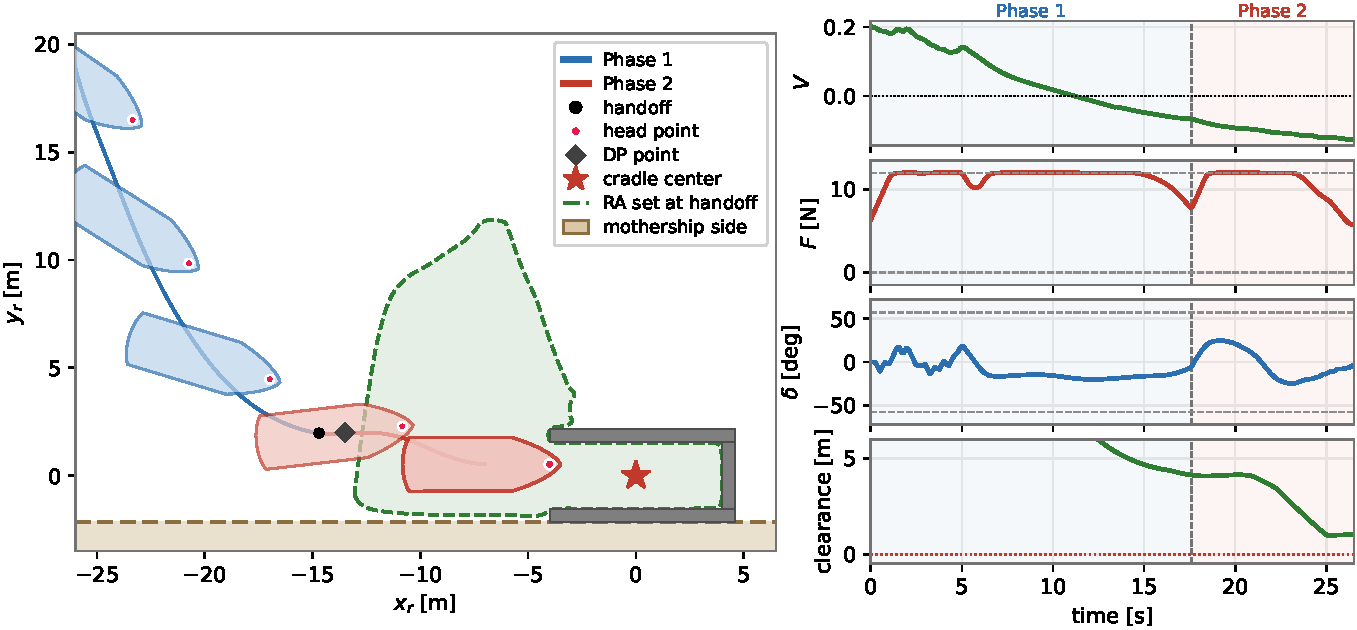
\includegraphics[width=0.92\linewidth]{fig/rep_run}
  \caption{Representative recovery of the proposed two phase policy. On the left the head point path in the cradle relative frame, with Phase 1 in blue and Phase 2 in red and the handoff marked. On the right the value $V$, the thrust $F$, the rudder $\delta$, and the clearance over time, where the thrust and the rudder stay within their amplitude limits and the clearance stays above zero.}
  \label{fig_representative}
\end{figure*}

\begin{figure*}[t]
  \centering
  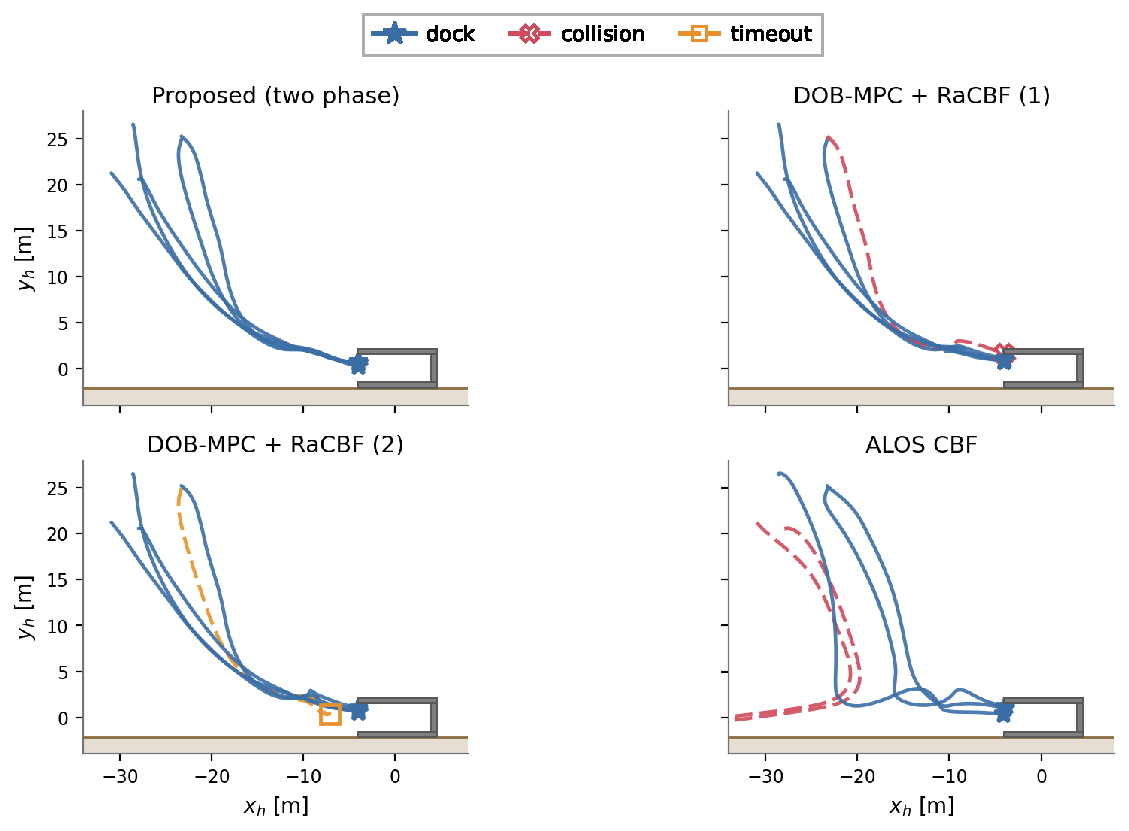
\includegraphics[width=0.86\linewidth]{fig/trajectories_montecarlo}
  \caption{Head point trajectories for five representative scenarios, the same five for every controller, in the cradle relative frame. Docks are solid with a star, collisions and timeouts are dashed with a cross and a square, and the cradle pocket and the mothership side boundary are drawn. The proposed policy docks all five, while each baseline shows its failure mode.}
  \label{fig_trajectories}
\end{figure*}

\begin{table}[t]
  \centering
  \caption{Monte Carlo comparison over 100 sea scenarios. Dock, collision, and timeout counts, the median recovery time, the worst case clearance to the obstacles, and the mean and worst per call computation time. The two barrier gains of the DOB-MPC with RaCBF baseline are labelled (1) and (2).}
  \label{tab_montecarlo}
  \resizebox{\linewidth}{!}{%
  \begin{tabular}{lcccccc}
    \hline
    Controller & Dock & Collision & Timeout & Median time [s] & Worst clearance [m] & Compute mean (max) [ms] \\
    \hline
    Proposed (two phase) & 100 & 0 & 0 & 33.0 & $+0.69$ & 0.6 (1.7) \\
    DOB-MPC + RaCBF (1) & 95 & 5 & 0 & 39.7 & $-0.003$ & 4.1 (16.0) \\
    DOB-MPC + RaCBF (2) & 98 & 0 & 2 & 41.6 & $+0.41$ & 4.0 (15.7) \\
    ALOS CBF & 69 & 16 & 15 & 48.3 & $-0.003$ & 4.2 (56.2) \\
    \hline
  \end{tabular}}
\end{table}

\begin{figure}[t]
  \centering
  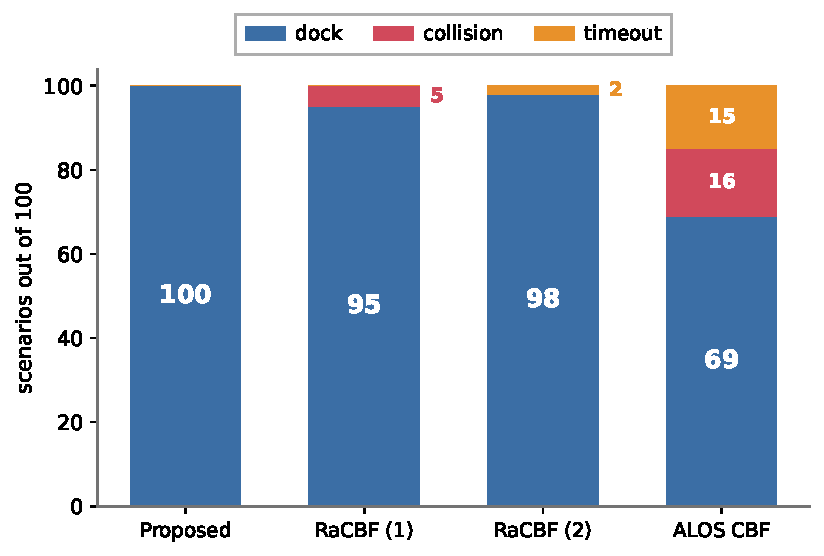
\includegraphics[width=0.92\linewidth]{fig/success_bar}
  \caption{Outcome of the 100 sea scenarios for each controller, counted as docks, collisions, and timeouts. The proposed policy docks every scenario, the barrier baselines a few less, and the ALOS CBF guidance far fewer.}
  \label{fig_success}
\end{figure}

\begin{figure}[t]
  \centering
  \includegraphics[width=\linewidth]{fig/value_wall_comparison}
  \caption{Learned reach avoid value slices trained without and with the mothership wall. The wall removes the false reachable region inside the mothership while leaving the free state set nearly unchanged.}
  \label{fig_wall_ablation}
\end{figure}

\subsection{Processor in the loop simulation}\label{sec_results_pil}

The trained policy was deployed on an embedded processor in the loop setup in which the plant was simulated on a host machine while the policy ran on the target hardware in floating point. The per step inference time of the actor network remained well below the 0.2 s control period at 5 Hz, leaving margin for the remaining guidance and navigation software. Two effects separate this deployment from the training environment. First, the round trip communication delay shifts the state on which the action is computed, and second, the zero order hold keeps the actuator rate command constant over the full period rather than updating it continuously. Because the policy commands actuator rates and the actuator states are part of the augmented state, both effects act as a bounded perturbation that the robust training already covers, and the recovery success rate observed in the processor in the loop campaign remained consistent with the numerical results of Section~\ref{sec_results_sim}. The measured timing statistics and the gap between the training environment and the embedded deployment are reported in Table~\ref{tab_pil} and Fig.~\ref{fig_pil_timeseries}.

\begin{table}[t]
  \centering
  \caption{Processor in the loop timing and performance. Actor inference time statistics, end to end loop latency, and recovery success rate compared with the training environment.}
  \label{tab_pil}
  \resizebox{\linewidth}{!}{%
  \begin{tabular}{lcc}
    \hline
    Quantity & Training environment & Embedded target \\
    \hline
    Inference time [ms] & & \\
    Loop latency [ms] & & \\
    Success rate & & \\
    \hline
  \end{tabular}}
\end{table}

\begin{figure}[t]
  \centering
  \includegraphics[width=\linewidth]{fig/pil_timeseries}
  \caption{Processor in the loop time histories of the actuator commands and states under the zero order hold, compared with the training environment on the same initial condition.}
  \label{fig_pil_timeseries}
\end{figure}

\section{Conclusion}\label{sec_conclusion}

This paper formulated the docking phase of USV cradle recovery as a robust discounted reach avoid problem, extending the discounted reach avoid backup to a bounded disturbance game whose fixed point under approximates the true reach avoid set and converges to it as the discount tends to one, and embedded the learned value in a certified two phase framework in which membership in the reach avoid set decides both the handoff from the approach controller and the fallback out of the docking phase. In Monte Carlo simulations against the worst case adversary the learned policy recovered the underactuated USV into the moving cradle with a high success rate and very few collisions, and it transferred to an embedded processor in the loop deployment within the control period, whereas the hand designed funnel barrier failed through actuator saturation under the same underactuation. The certificate is limited by the approximation error of the learned value and policy, and the method has not yet been validated in full scale sea trials, so future work will pursue verified error bounds on the learned set and experimental recovery campaigns at sea.

\section*{Acknowledgements}
This research was supported by the Ministry of Oceans and Fisheries, Republic of Korea.

\bibliographystyle{agsm}
\bibliography{bib}

\end{document}
